\documentclass[12pt,a4paper]{article}
\usepackage{bold-extra}
\usepackage{appendix}
\usepackage{amsfonts,amsmath,amssymb}
\usepackage{enumerate}
\usepackage{float}
\usepackage{geometry}
\usepackage{graphicx}
\usepackage{latexsym}
\usepackage{listings}
\usepackage{multicol,multirow}
\usepackage{subfigure}
\usepackage{tabularx}
\usepackage{ulem}
\usepackage{tikz}
\usepackage{xcolor}
\geometry{a4paper,left=1in,right=1in,top=1in,bottom=1in}
\begin{document}
\centerline{\Huge{{\textbf{PHYSICS I\ \ Problem Set 1}}}}
\vspace{0.5cm}
\leftline{\large{Name: Haotian Fu}}
\rightline{\large{Student ID: 520021910012}}
\paragraph{\large \textbf{Problem 1}}~{\textbf{Solution}}
\vspace{2mm}
\par{\normalsize We first have to estimate the population in Beijing. Just suppose population of Beijing (P) = 100 $\times 10^4$. Then since piano is not an instrument of cheap price, therefore even in Beijing we can estimate that every 100 people own one piano on average, noted as Amount of pianos per person (A) = $\frac{1}{100}$.}
\par For every piano, suppose it needs one tuning per year and one tuner can tune 100 times per year. Then for each piano, it needs $\frac{1}{100}$ tuner.
\par Therefore, we can calculate as follows.
\begin{align*}
	\text{tuners} = 100 \times 10^4 \times \frac{1}{100} \times \frac{1}{100} = 100 \ \text{(people)}
\end{align*}

\paragraph{\large \textbf{Problem 2}}~{\textbf{Solution}}
\vspace{2mm}
\par We here apply dimentional analysis. The unit of period is $s$.
\par The unit of density of mass is $kg/m^3$ while the unit of gravitational constant is $N\cdot m^2/kg^2$. In addition, we know that $N=kg\cdot m/s^2$. Therefore, we have the equation below.
\begin{align*}
	s = (\frac{kg}{m^3})^A \times (\frac{m^3}{kg\cdot s^2})^B
\end{align*}
\par Then solve this equation we get
\begin{equation*}
	\begin{cases}
		A=-\frac{1}{2}\\
		B=-\frac{1}{2}
	\end{cases}
\end{equation*}

\paragraph{\large \textbf{Problem 3}}~{\textbf{Solution}}
\vspace{2mm}
\par False.
\par We can consider one counter-example that \textbf{u} = (3,0) while \textbf{w} = (0,4). It is evident that $\lvert$\textbf{u}$\rvert$ = 3 $\textless$ $\lvert$\textbf{w}$\rvert$ = 4. However, $x_u$ = 3 $\textgreater$ $x_w$ = 0.
\par Therefore, the statement mentioned in problem 3 is false.

\paragraph{\large \textbf{Problem 4}}~{\textbf{Solution}}
\vspace{2mm}
\par (a) $\lvert$\textbf{$r_1$}$\rvert$ = $\sqrt{(4\hat{n_x})^2 + (3\hat{n_y})^2 + (8\hat{n_z})^2}$ = $\sqrt{89}$\ (m)
\par \ \ \ \ \ $\lvert$\textbf{$r_2$}$\rvert$ = $\sqrt{(2\hat{n_x})^2 + (10\hat{n_y})^2 + (5\hat{n_z})^2}$ = $\sqrt{129}$\ (m)
\vspace{2mm}
\par (b) $\lvert$\textbf{$r_{12}$}$\rvert$ = $\lvert$\textbf{$r_2$}$\rvert$ - $\lvert$\textbf{$r_1$}$\rvert$ = (-2$\hat{n_x}$,7$\hat{n_y}$,-3$\hat{n_z}$)
\vspace{1mm}
\par \ \ \ \ \ unit vector of \textbf{$r_{12}$} = $\frac{\textbf{$r_{12}$}}{\lvert\textbf{$r_{12}$}\rvert}$ = $\frac{1}{\sqrt{(-2\hat{n_x})^2 + (7\hat{n_y})^2 + (-3\hat{n_z})^2}}$ $\times$ (-2$\hat{n_x}$,7$\hat{n_y}$,-3$\hat{n_z}$)
\par \ \ \ \ \ \ \ \ \ \ \ \ \ \ \ \ \ \ \ \ \ \ \ \ \ \ \ \ \ = (-$\frac{\sqrt{62}}{31}\hat{n_x}$,$\frac{7\sqrt{62}}{62}\hat{n_y}$,-$\frac{3\sqrt{62}}{62}\hat{n_z}$)
\vspace{2mm}
\par (c) $\cos \measuredangle$(\textbf{$r_1$},\textbf{$r_2$}) = $\frac{\textbf{$r_1$}\cdot\textbf{$r_2$}}{\lvert\textbf{$r_1$}\rvert \cdot \lvert\textbf{$r_2$}\rvert}$ = $\frac{78}{\sqrt{11481}}$ = 0.728
\par \ \ \ \ \ $\cos \measuredangle$(\textbf{$r_1$},\textbf{$r_{12}$}) = $\frac{\textbf{$r_1$}\cdot\textbf{$r_{12}$}}{\lvert\textbf{$r_1$}\rvert \cdot \lvert\textbf{$r_{12}$}\rvert}$ = $\frac{-11}{\sqrt{5518}}$ = -0.148
\par \ \ \ \ \ $\cos \measuredangle$(\textbf{$r_2$},\textbf{$r_{12}$}) = $\frac{\textbf{$r_2$}\cdot\textbf{$r_{12}$}}{\lvert\textbf{$r_2$}\rvert \cdot \lvert\textbf{$r_{12}$}\rvert}$ = $\frac{51}{\sqrt{7998}}$ = 0.570
\vspace{1mm}
\par \ \ \ \ \ Therefore, we get
\par \ \ \ \ \ $\measuredangle$(\textbf{$r_1$},\textbf{$r_2$}) = $\cos^{-1}$ (0.728) = 0.755 (rad) = 43.3 ($^\circ$)
\par \ \ \ \ \ $\measuredangle$(\textbf{$r_1$},\textbf{$r_{12}$}) = $\cos^{-1}$ (-0.148) = 1.72 (rad) = 98.5 ($^\circ$)
\par \ \ \ \ \ $\measuredangle$(\textbf{$r_2$},\textbf{$r_{12}$}) = $\cos^{-1}$ (0.570) = 0.964 (rad) = 55.2 ($^\circ$)
\vspace{2mm}
\par (d) orthogonal projection vector of \textbf{$r_2$} onto \textbf{$r_1$} = $\frac{\textbf{$r_2$}\cdot\textbf{$r_1$}}{\lvert\textbf{$r_1$}\rvert}$$\cdot$$\frac{\textbf{$r_1$}}{\lvert\textbf{$r_1$}\rvert}$ = ($\frac{312}{89}$,$\frac{234}{89}$,$\frac{62
4}{89}$)
\par \ \ \ \ \ orthogonal projection of \textbf{$r_2$} onto \textbf{$r_1$} = $\frac{\textbf{$r_2$}\cdot\textbf{$r_1$}}{\lvert\textbf{$r_1$}\rvert}$ = $\frac{78}{\sqrt{89}}$ = $\frac{78\sqrt{89}}{89}$
\vspace{2mm}
\par (e) 
\begin{equation*}
\textbf{$r_{12}$} \times \textbf{$r_1$} = {
\left| \begin{array}{ccc}
1 & 1 & 1\\
-2 & 7 & -3\\
4 & 3 & 8
\end{array} 
\right |}
= (65\hat{n_x},4\hat{n_y},-34\hat{n_z})
\end{equation*}

\paragraph{\large \textbf{Problem 5}}~{\textbf{Solution}}
\vspace{2mm}
\par (a) No, uniform circular motion is a counter-example.
\par \ \ \ \ \ \ Suppose the uniform circular motion is two-dimensional, then \textbf{n} = ($\cos(\omega t)\hat{n_x}$,$\sin(\omega t)\hat{n_y}$).
\par \ \ \ \ \ Then \textbf{$\dot{n}$} = ($-\omega\sin(\omega t)\hat{n_x}$,$\omega\cos(\omega t)\hat{n_y}$), whose magnitude does not necessarily equal to one.
\vspace{2mm}
\par (b) Suppose \textbf{n} = ($x_1$,$x_2$,...,$x_n$). Then we have $\sum\limits_{i=1}^n$ $x_i^2$ = 1. We differenciate on both sides and get $\sum\limits_{i=1}^n$ $2x_i\cdot\dot{x_i}$ = 0, namely, $\sum\limits_{i=1}^n$ $x_i\cdot\dot{x_i}$ = 0, namely, \textbf{n} $\cdot$ \textbf{$\dot{n}$}.
\par \ \ \ \ \ Therefore, \textbf{n} and \textbf{$\dot{n}$} are perpendicular to each other.

\paragraph{\large \textbf{Problem 6}}~{\textbf{Solution}}
\vspace{2mm}
\par (a) $a_x$ = $\frac{dv_x(t)}{dt}$ = -$\frac{10}{3}e^{-\frac{t}{3}}$\ ($m/s^2$)
\par (b) According to (a), $\lvert$$a_x$$\rvert$ = $\frac{10}{3}e^{-\frac{t}{3}}$ $\textgreater$ 0 wherever t equals. Therefore, the particle will never stop, namely, \textit{t} $\rightarrow$ +$\infty$ when the particle stops.
\par (c) We may use improper integral to calculate the distance travelled, noted as \textit{s}.
\begin{align*}
s = \int_0^{\infty} 10e^{-\frac{t}{3}} = -30e^{-\frac{t}{3}} + \text{C} \vert_0^{\infty} = 30\ (m)
\end{align*}

\par (d) According to previous questions, we have 
\begin{align*}
a_x(t) &= -\frac{10}{3}e^{-\frac{t}{3}}\ (m/s^2)\\
v_x(t) &= 10e^{-\frac{t}{3}}\ (m/s)\\
x(t) &= -30e^{-\frac{t}{3}}+30\ (m)
\end{align*}
\par \ \ \ \ \ Graphs are shown below.
\begin{figure}[H]
    \centering
    \subfigure[$a_x(t)$ vs. $t$]{
    	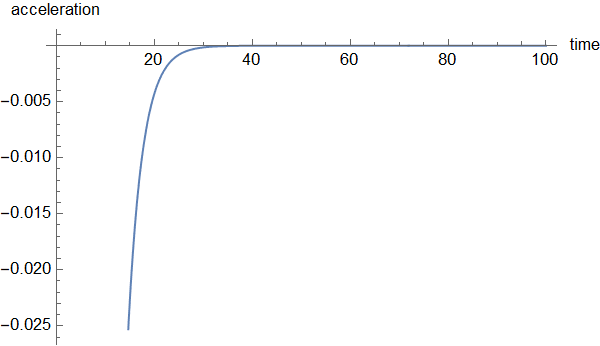
\includegraphics[height = 2.5cm]{1.png}
    }\hspace{5mm}
    \subfigure[$v_x(t)$ vs. $t$]{
    	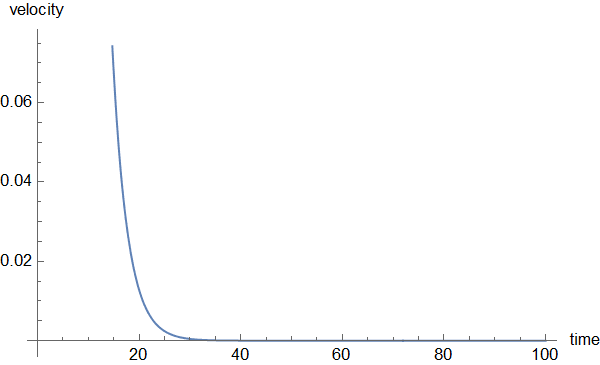
\includegraphics[height = 2.5cm]{2.png}
    }\hspace{5mm}
    \subfigure[$x(t)$ vs. $t$]{
    	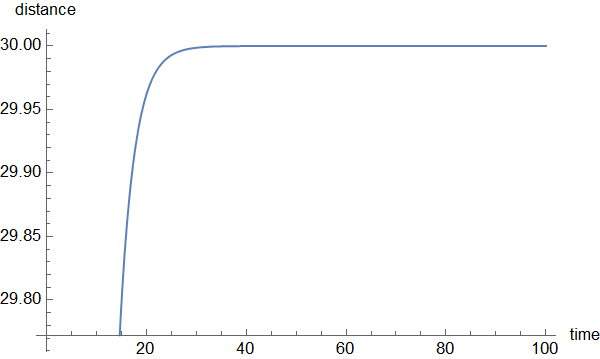
\includegraphics[height = 2.5cm]{3.png}
    }\hspace{5mm}
\end{figure}
\par (e) average velocity = $\frac{x(10)-x(0)}{10-0}$ = 2.89 ($m/s$)
\par \ \ \ \ Namely, the magnitude of average velocity is 2.89 $m/s$ while the direction of average velocity is the positive direction (along x-axis).
\par (f) average speed = $\lvert$ $\frac{x(10)-x(0)}{10-0}$ $\rvert$ = 2.89 ($m/s$)
\paragraph{\large \textbf{Problem 7}}~{\textbf{Solution}}
\vspace{2mm}
\par Suppose the velocity of padlling is $v_p$ while the velocity of river is $v_w$, and the distance of the river is $s$. Let A to B be the positive direction. Then according to the description, we have
\begin{equation*}
	\begin{cases}
		3(v_p+v_m) = s\\
		6(v_p-v_m) = s
	\end{cases}
\end{equation*}
\par Solve the equations we get
\begin{equation*}
	\begin{cases}
		v_p = \frac{s}{4}\\
		v_m = \frac{s}{12}
	\end{cases}
\end{equation*}
\par Therefore, the time needed if the tourist does not paddle is $t$ = $s$ / $v_m$ = 12 ($h$)

\paragraph{\large \textbf{Problem 8}}~{\textbf{Solution}}
\vspace{2mm}
\par Let the dropped paddle be the frame of reference (FoR). Then the speed of the fisherman is always his speed with respect to river.
\par According to the description, the total distance of the paddle travelled is 6 $km$ and at the time of 1 \textit{h}, the paddle must have travelled half of the total distance, i.e., 3 \textit{km}. Therefore, the speed of the river current is $\frac{3}{1}$ = 3 (\textit{km/h})
\end{document}